% !TeX root = ../../main.tex
\documentclass[../AAE590LGM_HW3.tex]{subfiles}
\begin{document}

\subsection{2.c) \textbf{Autonomous Error Dynamics:}}
\underline{Question}: \\
\textbf{Verify numerically:} Choose random $X, Y \in \SE{2}$ and a twist $\xi = (15, 0, 0.3)^T$. Compute both sides of the group affine equation and confirm agreement to machine precision. \\
\underline{Solution}: \\
Code snippet 1 shows the verification of group affine property of the $\SE{2}$ unicycle dynamics
\lstinputlisting[language=Python,caption={Unicycle Group Affine Test}, inputpath=../../../Tests/SE2]{test_SE2_group_affine.py}

\begin{figure}[H]
    \caption{Group Affine Unicycle Test Passing}
    \centering
    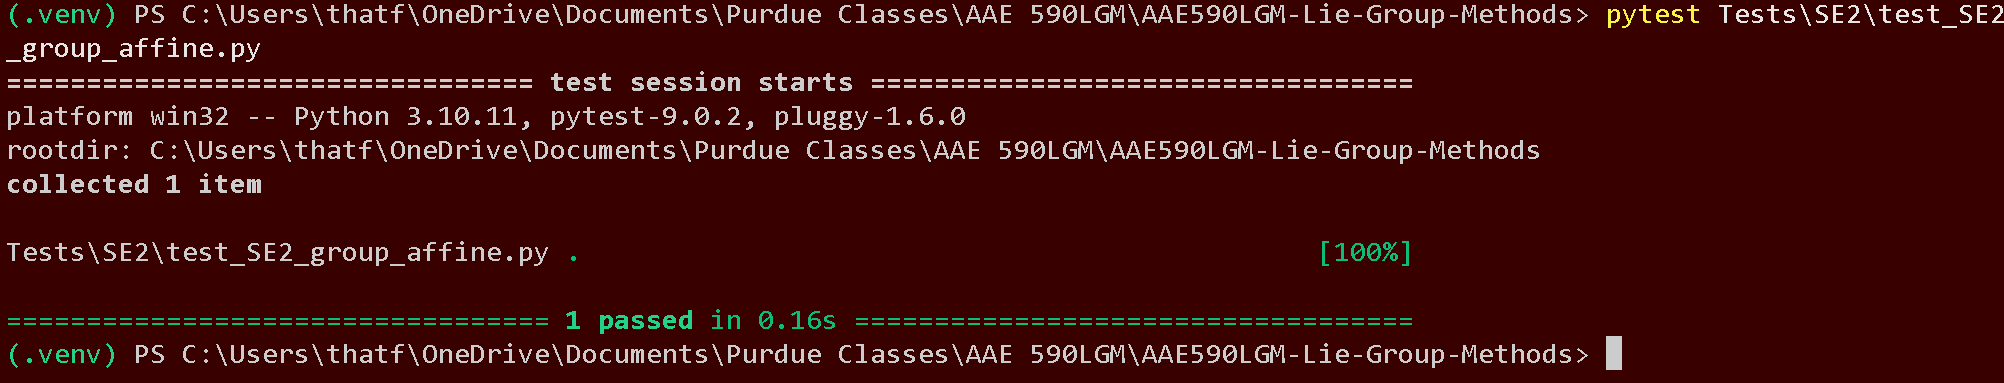
\includegraphics[width=0.7\linewidth]{AAE590LGM_HW3_Q2_gfckpass.png}
\end{figure}

\end{document}